%% ==============================================
%%                   Evaluation
%% ==============================================
%% Author: Fabian Sorn
%% ==============================================

\chapter{Evaluation}
\label{ch:Evaluation}

This chapter will focus on the evaluation of the framework. The biggest question
when it comes to evaluating performance of widgetmark is, how much overhead it
is adding compared to a standard application. The bigger our overhead is, the
more negative the results will be compared to the realistic value we can expect.
To evaluate the accuracy of our benchmarking framework, we will compare the
times measured in a simple example use case with an actual implementation as a
minimal PyQt application. This application will only house a single plot updated
by the same conditions as the use case. To measure the timing in the
application, we will record a timestamp after each update. To find out how the
overhead of the framework develops under different load scenarios, we will use
different dataset size parameters for the plotting. For the evaluation we will
only choose a single plotting library, which will be PyQtGraph.

Table \ref{tab:evaluation} compares the measured frame rates for each use case.
Both variants were executed on the same hardware with the same screen resolution
as well as the same window size. The measured data shows a trend of the
framework being slightly slower compared to the minimal PyQt application, which
is only slightly bigger than the often measured fluctuation between the
execution of different use cases.

\begin{table}[h]
\begin{center}

\captionof{table}{
    Frame rate comparison between widgetmark and a minimal PyQt application
}
\label{tab:evaluation}

\begin{tabular}{rrr}

\hline
Dataset Size & Widgetmark & PyQt Application \\
\hline
1000         & 58.8       & 59.8             \\
10000        & 59.7       & 59.6             \\
500000       & 23.8       & 25.9             \\
1000000      & 12.5       & 13.9             \\
\hline

\end{tabular}
\end{center}
\end{table}

While these measurements already provide us with a general trend of the
framework adding a small overhead to our execution, it raises the question, how
this deviation compares with the fluctuation of the recorded times within a
execution. To compare this we first will have to get access to all measured
delta times for the PyQt application as well as the widgetmark run.

As a small rehearsal, we will quickly explain the sizes used in the following
detailed evaluation and why they are meaningful for us. The first important
measurement is the delta timing $\Delta t$, which describes the difference
between two measured adjacent time stamps. From a set of $m$ timestamps it can
be calculated for two adjacent timestamps $t_{i+1}$ and $t_i$ as:

$$\Delta t_{i} = t_{i+1} - t_{i}$$

The arithmetic mean or average $\bar{\Delta t}$ describes the average from our
set of $m-1$ measured delta times and is defined as:

$$\bar{\Delta t} = \frac{1}{m-1} * \sum_{i=0}^{m-1} {\Delta t_{i+1} - \Delta t_{i}}$$

The standard deviation $\sigma$ of our delta times describes, how far most
values are deviated from $\bar{\Delta t}$. From the standard $\sigma$ we can get
a better idea if the measured times are very consistent or if they differ much
from each other. It is defined as:

$$ \sigma_{\Delta t} = \sqrt{\frac{1}{m-2} * \sum_{i=1}^{m-2} (\Delta t_{i} - \bar{\Delta t})^2} $$

The range of a set of $m-1$ delta times $\Delta t_i$ describes the difference
between the largest and smallest measured $\Delta t$ and is defined as:

$$R_{\Delta t} = \Delta t_{max} - \Delta t_{min}$$

Figures \ref{a:tab:evaluation:1000}, \ref{a:tab:evaluation:10000},
\ref{a:tab:evaluation:50000} and \ref{a:tab:evaluation:100000} compare all
measured delta times in the widgetmark as well as the minimal PyQt application.
For smaller dataset sizes, there are only small difference between both
noticeable. If the dataset size however increases, the difference measured in
the frame rates can be seen very well. In figure \ref{fig:evaluation:avg}, which
shows the average of the measured delta times, this difference becomes more
apparent. Compared to the standard deviation within a set of measured delta
times, the difference between both $\bar{\Delta t}$.

\begin{figure}[h]
    \centering
    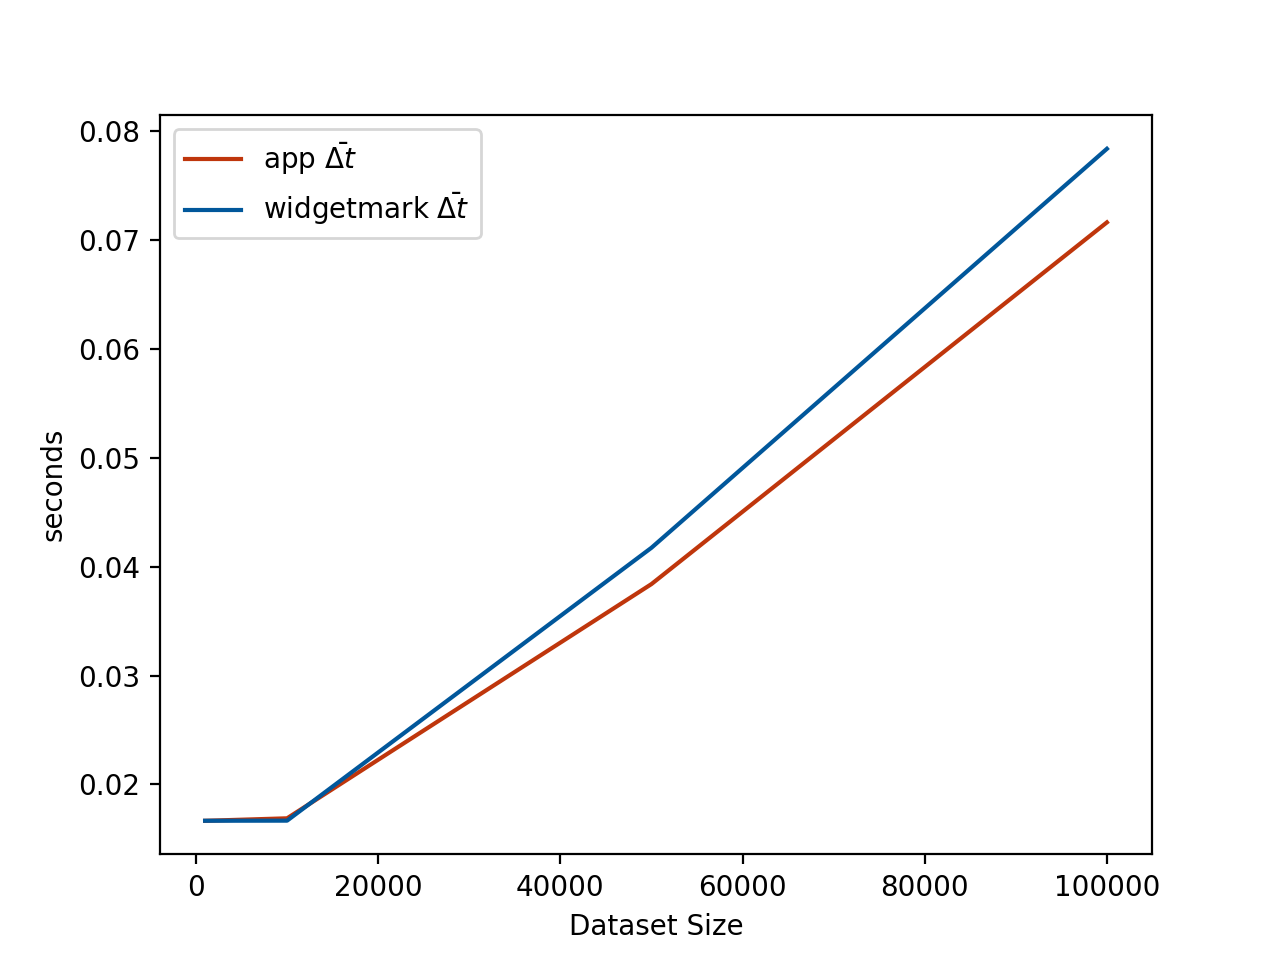
\includegraphics[width=12cm]{resources/img/evaluation/Eval_AVG}
    \caption{Average delta timing between both execution variants}
    \label{fig:evaluation:avg}
\end{figure}

Figure \ref{fig:evaluation:std} compares the difference between the average
delta times, the fluctuation of measured individual delta times and the ranges
$R_{\Delta t}$ of the framework as well as the minimal application. The
difference between widgetmark and the app in $\bar{\Delta t}$ is bigger compared
to their individual standard deviations $\sigma_{\Delta t}$, but much smaller
than their value ranges $R_{\Delta t}$.

\begin{figure}[h]
    \centering
    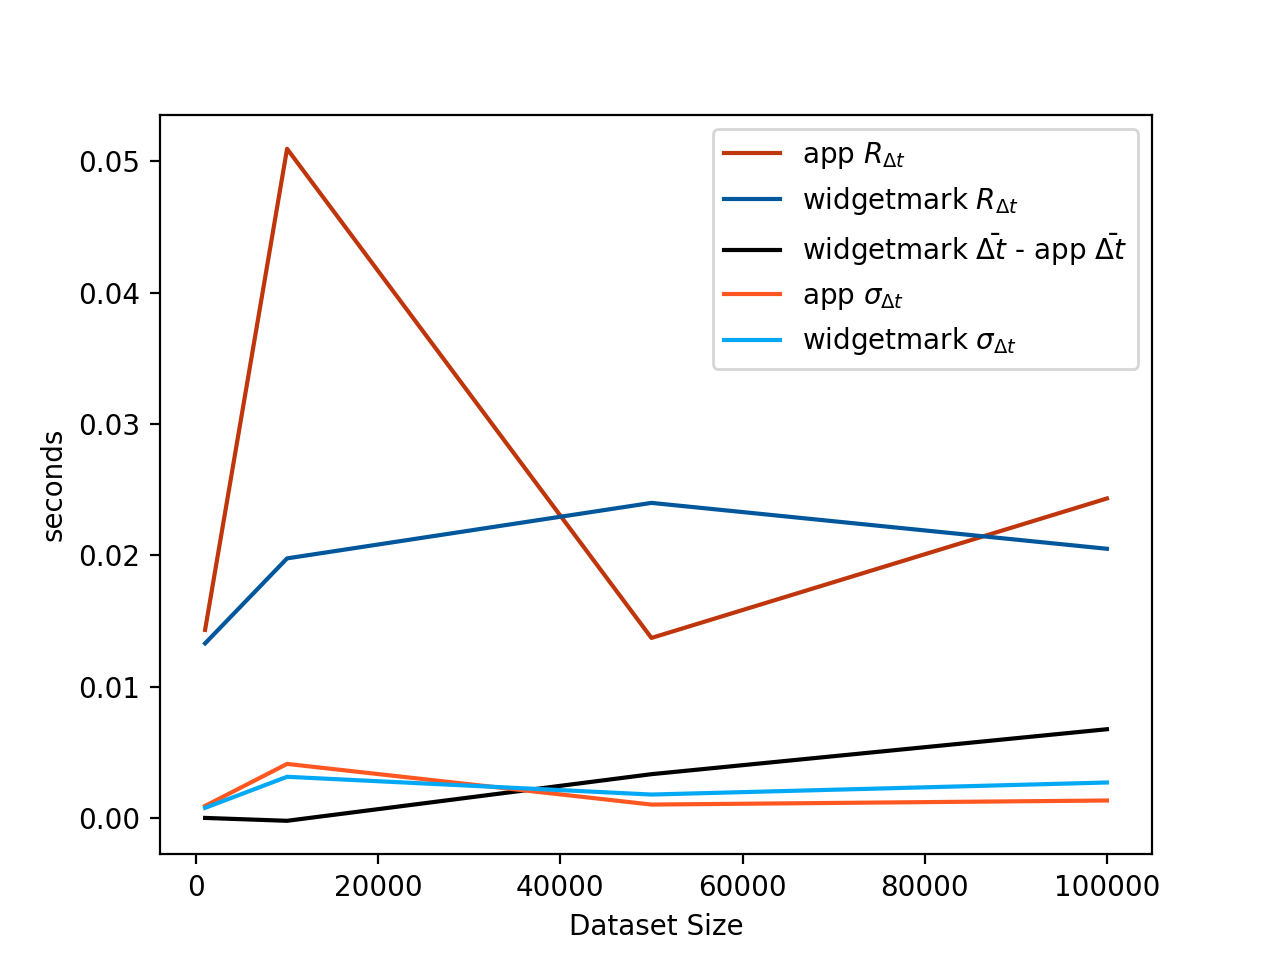
\includegraphics[width=12cm]{resources/img/evaluation/Eval_STD}
    \caption{Standard deviation compared to the delta timing value ranges and
        the average delta timing difference between both execution variants}
    \label{fig:evaluation:std}
\end{figure}

As a summary for the evaluation you can say, that widgetmark does add a slight
overhead to the executed use case. This overhead however does only slightly
influence the outcome of each use case, since it is still manages to represent
the libraries realistic performance capabilities.
